\section{Approach}
\label{cp5:approaches}


We explore three approaches to automatically identify text that is relevant to a particular software task.
These approaches encompass lexical similarity, word semantics, and frame semantics and are detailed later in this section.



All approaches take a task and a pertinent artifact as inputs and output the sentences 
that are most likely to contain information that assists a developer in completing their task. 
To determine how many sentences an approach should identify, we consider that 
no more than 20\% of the content in the artifacts in the
 \acs{DS-synthetic} and the \acs{DS-android} corpora are deemed relevant to a task, which, on average, accounts for 8.93 sentences. 
We approximate these values to a target number of 10 sentences per input task-artifact. 
Our decision to output a certain number of sentences regardless of the approach is to have an easy framework for their comparison (Section~\ref{cp5:evaluation}).



\subsection{Lexical Similarity}

As a baseline, we use Vector Space Model (VSM)~\cite{Salton1975vsm} from Information Retrieval~\cite{Manning2009IR}
to compute the lexical similarity between the sentences within a pertinent artifact and a task. 
Using this model, we can identify the sentences with highest lexical similarity 
as the ones most likely to contain information relevant to the input task.




VSM represents both a task and individual sentences within an artifact as vectors of term weights,
where the weight of a term
can be computed using a Term-Frequency Inverse-Document-Frequency scheme---\textit{tf.idf} accounts for how frequent a term is in an artifact (\textit{tf}) as well as how 
unique that term is across an entire corpora (\textit{idf})~\cite{Manning2009IR}. 
\red{provide formulas for tf idf}


Once we obtain vector representations $t$ and $s$ 
for an input task and an arbitrary artifact sentence, 
their lexical similarity can be computed 
using the cosine similarity between their vectors, as Equation~\ref{eq:lex-sim} shows:



\begin{equation}
    cos(t,s) = \frac{t^Ts}{\|t\| \|s\|}
    \label{eq:lex-sim}
\end{equation}
\smallskip

By ranking the sentences in an artifact according to their similarity scores, i.e., from highest to lowest,
we can  select the top-n sentences as the ones relevant to an input task.




\subsection{Word Semantics}


Language models capture words' semantics based on the context in which words appear~\cite{harris1954distributional}.
They allow a more ``human-like reasoning'' even when words are lexically different, as in 
inferring that both the words \textit{king} and \textit{queen} are semantically similar and that they represent \textit{royalty}~\cite{Mikolov2013}.


% Considering that language models make sense of words in the same way that a human reader does~\cite{Just1980},
Considering how language models provide a semantic representation for words, we pose that we can identify task-relevant text by semantically matching the text in a pertinent artifact to the text in a task.
To this end, we first introduce general concepts needed to understand language models\footnote{
    For a in-depth overview of the concepts behind language models, please refer to Zhang et al.~\cite{zhang2021deep-learning}.
} and then, we detail how we use a baseline model~\cite{Mikolov2013} and also a state-of-the-art model~\cite{Devlin2018Bert} to automatically identify task-relevant text.





\subsubsection{Background}


% introduce language models
A core concept of a language model is Harris' distributional hypothesis~\cite{harris1954distributional}, which states that words that appear in a similar context tend to have similar meanings.


A language model exploits this hypothesis by building vector representations, namely \textit{word embeddings}, for each of the words in a text corpus.
For that, it requires a significantly large number of sentences so that
the model associates similar vector embeddings to words that are similar in meaning based on their context~\cite{Ye2016}. 

% Overview of baseline model
\smallskip
\begin{hangparas}{.0in}{0}
    {\small \textbf{ Skip-gram model.}} One common challenge to language models is that they need to learn word vector representations that are good at predicting the nearby words at low computational costs, e.g., the time needed to train a model, the model size, etc.
    The \textit{Skip-gram} model~\cite{Mikolov2013}, proposed by Mikolov et al., addresses such challenges using simple yet efficient training procedures. As Figure~\ref{fig:skip-gram-example} illustrates, the model learns vector representations by \textit{(i)} looking at the $n$ words that preceded and succeed word $w_t$
     as positive training examples, and by \textit{(ii)} randomly sampling words that do not appear in the same context as negative training examples. Empirical results have shown that negative sampling allows for an accurate model able to handle noise data and that 
     the vector representations provided by the model could be used to improve many natural language processing tasks~\cite{mikolov2013efficient}.
\end{hangparas}



\begin{figure}[H]
    \centering
    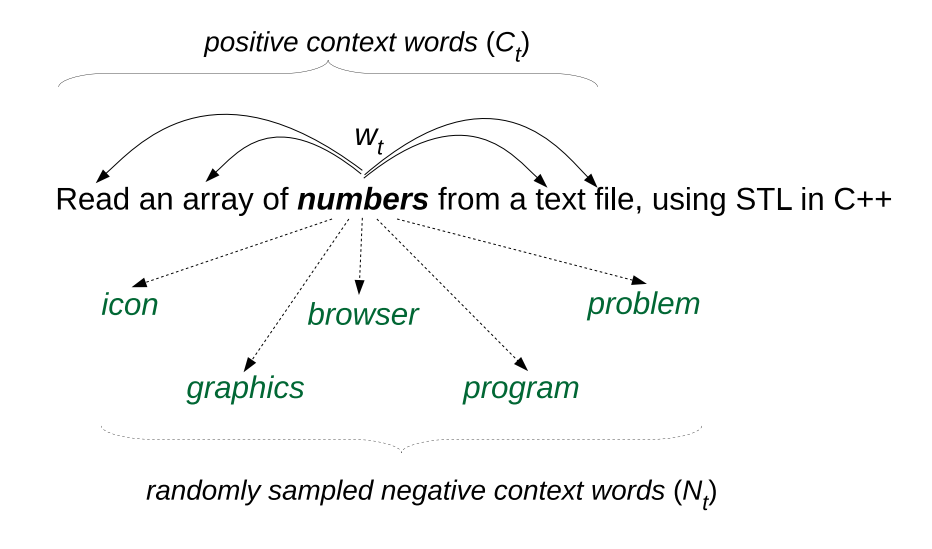
\includegraphics[width=.65\linewidth]{fig/cp5/ye-skip-gram-example}
    \caption{Positive and negative training examples in the Skip-gram model. Figure from~\cite{Ye2016}}
    \label{fig:skip-gram-example}
\end{figure}



Using the skip-gram model, one can identify that words $t$ and $s$ are semantically similar 
computing the cosine similarity between their corresponding word embedding representations ($w_t$ and $w_s$):



\begin{equation}
    cos(w_t,w_s) = \frac{w_t^Tw_s}{\|w_t\| \|w_s\|}
    \label{eq:word-sim}
\end{equation}






% Overview of state-of-the-art model
\smallskip
\begin{hangparas}{.0in}{0}
    {\small \textbf{BERT model.}} Context in the Skip-gram model refers to the positive/negative examples used during the model's training procedures; this however, does not allow the model to disambiguate words based on their surrounding text. In other words, a Skip-gram model will have a single vector representation for the word \textit{company} even when it can have different meanings, i.e., a business organization or being in the company of someone. In contrast, state-of-the-art models, such as \textit{BERT}~\cite{Devlin2018Bert}, provide different representations for the same word based on the sentence in which a word appears.
    This additional layer allows for more complex operations, such as word disambiguation \red{ref}.
\end{hangparas}

% builts on top of several other studies in the natural language processing and deep learning communities \ref{ref ELMo, Transformer, Attention} and the model

BERT also addresses tasks that need to understand relationships between sentences, which is a task not directly captured by language modeling~\cite{Devlin2018Bert}.
To capture sentence relationships, BERT training procedures consider both next word prediction---as in any language model---and also next sentence prediction, i.e., given a pair of sentences $A$ and $B$ the model 
is trained to predict the likelihood that sentence $B$ succeeds $A$ (Figure~\ref{fig:BERT}). 


\begin{figure}
    \centering
    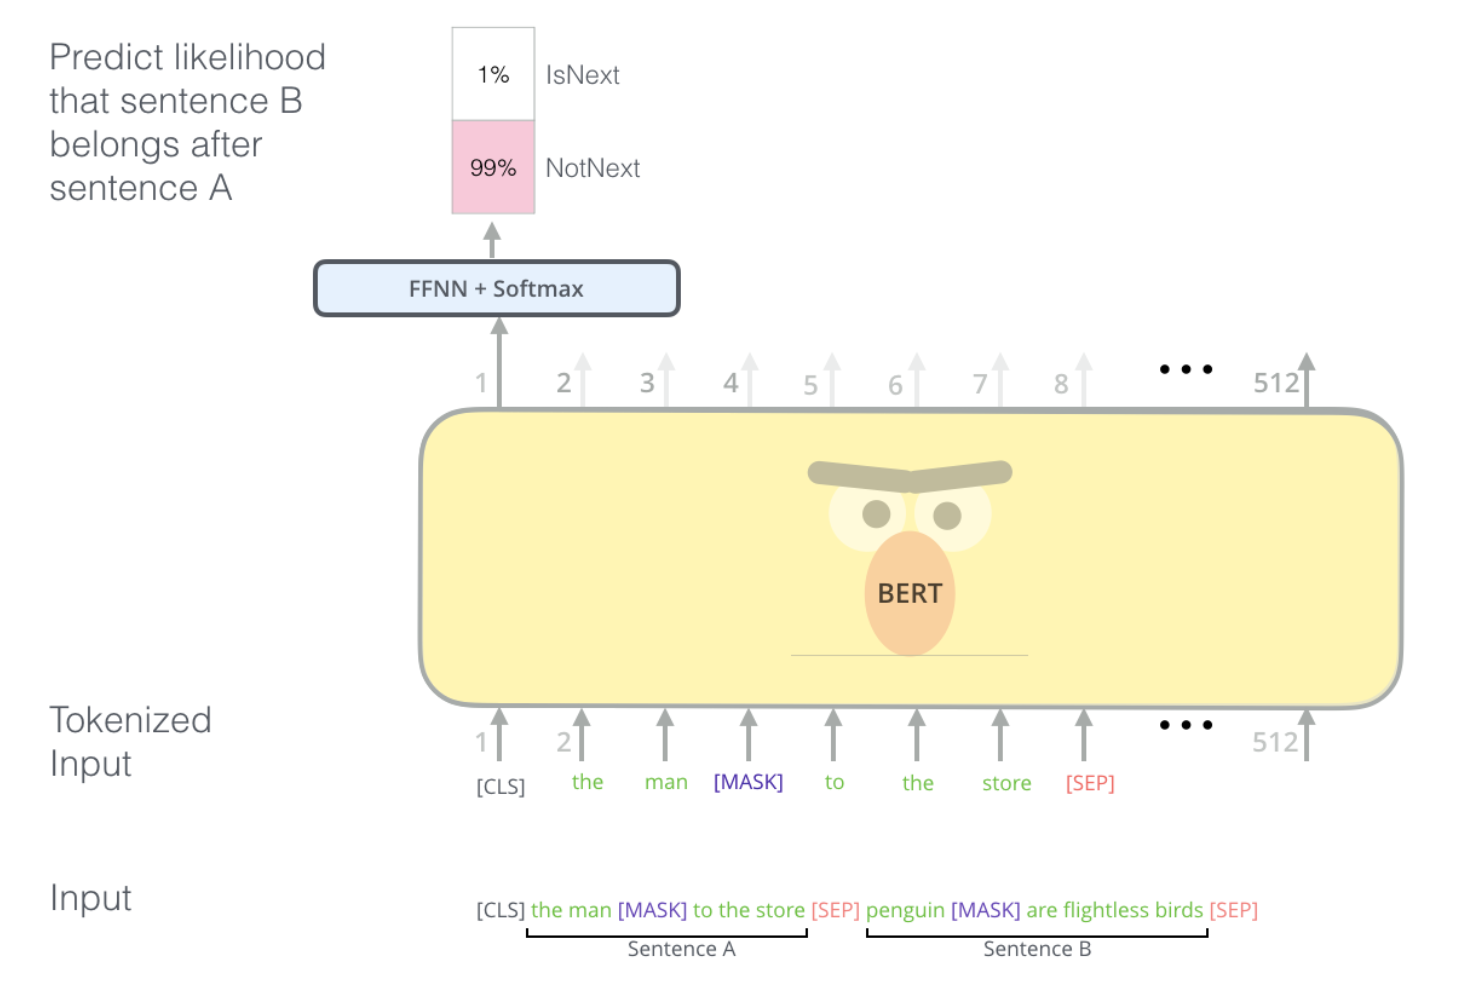
\includegraphics[width=.75\linewidth]{fig/cp5/BERT}
    \caption{BERT sentence prediction training procedures \red{(temporary)}}
    \label{fig:BERT}
\end{figure}



Since BERT addresses both next word prediction and next sentence prediction, the model can be used for several two-sentences tasks such as  question answering or natural language inference. Through sentence relationships, 
We pose that the model can be used to determine the relevance of a sentence based on an input software task.





\subsubsection{Semantic Similarity}






To compute the semantic similarity between the sentences within a pertinent artifact and a task,
we use the Skip-gram model~\cite{Mikolov2013} with word embeddings specifically trained for the software engineering domain~\cite{Efstathiou2018}.
Analogous to lexical similarity,  we can identify the sentences with highest semantical similarity 
as the ones most likely to contain information relevant to the input task.



Note that, since word embeddings provide vector representations at the word level, we compute vector representations 
at the sentence level by averaging the sum of the word embeddings of some input text.
Provided that we have sentence-level embeddings $w_t$ and $w_s$ for the text 
of an input task and an arbitrary artifact sentence, 
their semantic similarity can also be obtained 
using the cosine similarity: 





\subsubsection{BERT}





% https://jalammar.github.io/visualizing-neural-machine-translation-mechanics-of-seq2seq-models-with-attention/
% https://jalammar.github.io/illustrated-transformer/
% https://lilianweng.github.io/lil-log/2018/06/24/attention-attention.html


% At the time of their introduction, language models primarily used recurrent neural networks (RNN) and convolutional neural networks (CNN) to handle NLP tasks.




% By looking at all surrounding words, the Transformer allows the BERT model to understand the full context of the word, and therefore better understand searcher intent.

% This is contrasted against the traditional method of language processing, known as word embedding, in which previous models like GloVe and word2vec would map every single word to a vector, which represents only one dimension, a sliver, of that word's meaning.






% Look at the set of encoder hidden states it received – each encoder hidden states is most associated with a certain word in the input sentence
% Give each hidden states a score (let’s ignore how the scoring is done for now)
% Multiply each hidden states by its softmaxed score, thus amplifying hidden states with high scores, and drowning out hidden states with low scores




\subsection{Sentence Semantics}



\clearpage


